\documentclass{book}
\usepackage{mathtools}
\usepackage{tikz}
\usepackage{tikz-cd}
\usetikzlibrary{positioning}

\usepackage{amsthm}
\usepackage{amsmath}
\usepackage{amssymb}

\newtheorem{defn}[equation]{Definition}
\newtheorem{coro}[equation]{Corollary}
\newtheorem{prop}[equation]{Proposition}
\renewenvironment{proof}{\emph{Proof}}{\qed}


\begin{document}






\tableofcontents

\clearpage







\section{Foreword}
In transitioning to advanced classes, a physics student will find their familiar mathematical tools are inadequate to describe certain physical phenomena. The methods of traditional vector calculus in three dimensions, though very useful in electromagnetism and classical mechanics, are not always usable in higher dimensions, such as those used in general relativity and Hamiltonian mechanics. For that, we need differential geometry. When trying to learn a subject in mathematics, however, you tend to find books written for mathematicians, in a language that mathematicians are familiar with. As such, they are filled with long, obtuse definitions and prose that, while mathematically very precise, isn't exactly light reading, and can even be overkill for a proper physical understanding. 

When mathematicians write for mathematicians, they develop and motivate their mathematical tools for the purposes of ease of calculation and proofs. There is, of course, nothing wrong with this. Mathematicians ought to be writing for mathematicians, and we shouldn't try to force the constraints of our field on theirs. For physicists, however, proofs and ease of calculation are not the fundamental problems. Rather, we are trying to mathematically codify, organize, and characterize physical phenomena. The math that we use, therefore, ought to be entirely physically motivated. When the math is developed properly for our purposes in physics, there shouldn't be any "purely mathematical" constructs without an actual physical meaning. We do not claim that we have fully achieved this goal here,\footnote{This is the greater goal of the Foundations of Physics project as a whole} as there are open, unresolved problems in our work here, which will be addressed here when appropriate. 
What follows is a purely physical treatment of differential topology used in physics. While it is less mathematically rigorous than a typical math textbook, the hope is that the reader will be able to gain a geometric intuition for the math they use, so that the math isn't simply a black box beyond understanding, and that further study in the subject will be aided by a solid grounding here. Furthermore, by clarifying the underlying physical assumptions that we are working with at each step of the way, we will be more certain of the physical meaning of each of our mathematical tools, as well as the results we are able to derive.  The focus is always on readability, applicability, and physicality.


When we say "physical", we refer to properties and characteristics that we can directly measure in a laboratory. This definition is, at the moment, up for refinement though. Every tool we have in physics will at some level be an abstraction. Even something as simple as measuring mass will be to a certain extent "nonphysical." We cannot say, for instance, that an object in our laboratory is \emph{precisely} 5 kg, as our precision depends on the tools that we are using. We can say that it is 5 $\pm 0.01$ kg, but this error isn't a quantity that we directly measure. It would also not be correct to say that it is purely a mathematical abstraction. It is a result of the fact that our measurements are not infinitely precise. 

We assume on the part of the reader a class in introductory classical mechanics and electromagnetism, as well as vector calculus. More advanced topics in physics and mathematics may be touched on, but only for the use of giving an example, or demonstrating the usefulness of these mathematical tools. 


\chapter{Mathematical representations of physical objects}



\section{Physical objects and quantities}

At the heart of scientific investigation is the identifying and organizing of objects based on their properties, through measurement and experiment. This could be anything from setting a block on a scale to determine its weight to determining the species that a particular animal belongs to. For our purposes here, we will be dealing only with properties that can be described using real numbers, such as mass, temperature, velocity, etc. Identifying an object with a property involves first deciding which cases are possible and which are not. For example, when placing an object on a scale, you will not get a negative number (assuming, of course, that the scale has been properly zeroed). So, we have a set $U$, which the possible values the physical property can take on are contained in. The identification of a particular physical property with a real number is a \textbf{quantity}.

\begin{defn}
	A \textbf{quantity} is a function $q : U \to \mathbb{R}$ that assigns a measurable value to a physically possible case.
\end{defn}



It's possible, however, that one single quantity won't be enough to fully characterize an object. This presents an issue when trying to distinguish two objects. Say, for instance, that we're talking about weather. Knowing what the temperature will be tomorrow is certainly useful, but as anyone from Florida can tell you, 80$^o$F with 95$\%$ humidity is very different from 80$^o$F with 30$\%$ humidity. In characterizing objects, then, we will often want to define more than one quantity. By defining enough quantities to fully characterize one object, but not so many such that we have redundancies, we can define a \textbf{coordinate system}.



Normally, we think of coordinate systems in the context of quantifying an object's position, in terms of its x-, y-, and z-coordinates. Though it may be an abuse of terminology, we will use the same phrase to describe coordinates in other contexts. Consider, for instance, phase space. Configurations in phase space are fully characterized by position and momentum, which would be our two quantities, thus giving us a coordinate system. As another example, we can look at a system described by the ideal gas law. In this case, we would create a coordinate system with pressure, volume, and temperature. 

\begin{defn}
	A \textbf{coordinate system} $Q$ is a collection of $n$ quantities $q^i : U \to \mathbb{R}^n$ such that there is a one-to-one relationship between the physical objects in $U$ and elements of $\mathbb{R}^n$.
\end{defn}



With coordinate systems now defined, we recognize that in many instances, two different coordinate systems function just as well to describe a certain object. Mathematically, this occurs when two sets, each with defined coordinate systems, overlap. The points that lie within this overlapping section may be described in either coordinate system. To give an example from geography, consider an atlas of the world: a collection of maps. Depending on the atlas you're looking at, certain places may show up in multiple maps. Consider Moscow, for instance. It could very well show up on a map of Asia, perhaps in a square labeled B2, while also showing up on a map of Europe, perhaps in a square labeled C8. Either way of describing Moscow's position is equally valid, and you can freely "transform" between the coordinate systems as far as Moscow is concerned. Alternatively, consider the "point" Lisbon. Lisbon will show up on a map of Europe, perhaps in square F1, but you would never find Lisbon on a map of Asia. Therefore, its position may only be described in terms of the coordinates on the map of Europe.


\begin{defn}
	Given two coordinate systems  $Q : U \to \mathbb{R}^n$ and $Q' : V \to \mathbb{R}^n$ such that $U \cap V \neq \emptyset$, we call a \textbf{coordinate transformation} the function $f = Q' \circ (Q)^{-1} : \mathbb{R}^n \to \mathbb{R}^n$ (Figure 1.1).
\end{defn}




\begin{figure}[h]
\begin{center}
\begin{tikzcd}
	U \arrow[r, "Q", leftrightarrow] \arrow[d, "U \cap V" left, leftrightarrow] & \mathbb{R}^n \\
	V \arrow[r, "Q'", leftrightarrow] & \mathbb{R}^n \arrow[u, leftrightarrow]
\end{tikzcd}
\end{center}
\caption{This is a commutative diagram that shows how sets relate to each other, and what functions are used to relate them. The double sided arrows denote a one-to-one relationship between the elements of the two sets related using the operation above the arrow}
\end{figure}


Because of the poles, every location on Earth cannot be equally quantified with only one set of coordinates. This can be plainly seen on a typical flat map, such as a Mercator Projection. The most immediately obvious result of this flattening is that land proportions grow the closer to a pole they are, making Greenland appear massive, and the Sahara proportionally far smaller. The more important, but perhaps more subtle, outcome is that because the poles have in a sense been unraveled, the South Pole, which ought to be a single point, is an entire line along the southern edge of the map. A projection of the Earth onto a flat surface, such that one point on the Earth maps to one point on the surface, requires at least two separate maps. For instance, you could have a map of the top hemisphere, centered at the north pole, and then of the bottom hemisphere, centered at the south pole. From the Earth, then, we define \textbf{manifolds} as the general object that we project onto flat space. 


\textbf{Insert a picture of the Mercator Projection}

\textbf{Insert pictures of "polar" projections}

\begin{defn}
	A \textbf{manifold} is a set of physical objects $X$ such that for any $x \in X$ there exists a $U \subset X$ that contains $x$ and upon which a coordinate system $Q$ is defined. Manifolds have dimensionality, as determined by the dimension of their coordinate systems.
\end{defn}


Earlier, weather was given as an example of a set of possible cases of a system, with readings such as temperature and humidity allowing us to define a coordinate system. In this context, the "manifold" would be the set of possible weather configurations, with each point being a single weather report. Another example of a manifold would be the possible results of a blood drawing. The doctor takes your blood for analysis, the results of which are collected on a report, detailing things such as blood pressure, cholesterol levels, white blood cell count, etc. Each point on that manifold, therefore, would be a specific combination of blood pressure, cholesterol, and so forth. Further examples include: 

\begin{itemize}
\item The conditions of your car, with the dials on the dashboard being your method of reading them 

\item The freight on a ship, with the bill of lading detailing amounts

\item Any sort of information that can be condensed down to a series of real numbers

\end{itemize}

The variety of examples is to show the ubiquitousness of manifolds, and that they are very familiar, everyday objects. This versatility proves their usefulness in physics, and in scientific investigation in general. But unlike in the case of the Earth, manifolds do not in general come prepackaged with a notion of distance. What does it mean, for instance, for there to be distance between weather reports? Perhaps you can argue that distance comes into play by specifying where exactly the weather report was taken, but this is simply the geography example again under a different name. No, defining distance on manifolds requires first the definition of a particular mathematical structure, which we will not be addressing here. 




\section{Sub-manifolds and k-surfaces}

Consider again the weather report example, where we are taking into account where exactly the report was taken. Perhaps we decide to hold fixed where the weather report is taken (thereby making specification of the location redundant when comparing different readings). This takes us immediately from one manifold to another, where the latter has fewer dimensions than the former, and where any point on the latter is also a point on the former. Thus, geography is a \textbf{submanifold} of the weather report.


\begin{defn}
	Consider a manifold X of dimension n, and a manifold Y of dimension k, such that $k \leq n$. Y is a \textbf{submanifold} or a \textbf{k-surface}\footnote{In general, we will be using the term "k-surface", instead of "submanifold." There will be many terms throughout this thesis prefaced by "k-". In general, this means that the object in question has k dimensions, and can be organized by their dimensionality.} of X if any point on Y is also a point on X (Figure 1.2). 
\end{defn}


\begin{figure}[h]
\begin{center}
\begin{tikzcd}
X \arrow[r, "Q", leftrightarrow] & \mathbb{R}^n \\
Y \arrow[r, "Q|_Y", leftrightarrow] \arrow[u, hook] & \mathbb{R}^k \arrow[u, hook]
\end{tikzcd}
\end{center}
\caption{$Q|_Y$ is restriction notation. It means that it is the function $Q$ mapping between $X$ and $\mathbb{R}^n$, but restricted to map only from $Y$ to $\mathbb{R}^k$. We can use this notation as $Y$ and $\mathbb{R}^k$ are subsets of $X$ and $\mathbb{R}^n$, respectively.}
\end{figure}


\begin{defn}
	For some manifold X of dimension n, $S^k$ is the set of all possible \textbf{k-surfaces} of dimension $k \leq n$, and S $=$ $\cup^n_{k=0}S^k$ is the set of all surfaces. 
\end{defn}


We can go even further in our description of k-surfaces. First, we can hold certain quantities fixed, and vary the others. For instance, say we allow only one quantity to vary, while holding the others fixed. In the weather example, we could vary only temperature, holding all other properties fixed. On the manifold containing all weather reports, this varying of temperature would manifest itself as a line on the manifold, the points on which being weather reports whose values for all quantities besides temperature are identical. 
\begin{defn}
	A \textbf{coordinate line} is the set of points in $\mathbb{R}^n$ obtained by allowing one quantity to vary and holding the others fixed. 
\end{defn}

This same process can be done with any arbitrary number of fixed and varying coordinates. In general, a surface formed through the varying of coordinates is a \textbf{coordinate k-surface}. 

\begin{defn}
	A \textbf{coordinate k-surface} is the set of points in $\mathbb{R}^n$ obtained by allowing k quantities to vary and holding (n-k) quantities fixed.  
\end{defn}

When varying coordinates to creates coordinate lines, surfaces, volumes, etc., the varying can be brought to a halt by the geometry of the object that we're working on. Where the varying ends lies the \textbf{boundary} of our surface. Suppose our manifold is the Earth (the entire Earth, not just the surface). If we assume that we can freely move through the entirety of the Earth's crust, but may not leave the surface of the Earth, we may say that the Earth manifold has a boundary, that being the surface of the Earth. Because radius is held fixed on the surface, the boundary of the Earth has a dimensionality of 2, instead of 3. 

\begin{defn}
	Given k-surface $\sigma^k \in S^k$, the \textbf{boundary} of $\sigma^k$, denoted by $\partial\sigma^k \in S^{k-1}$ is the limit of varied coordinates. Points lying on the boundary are called \textbf{boundary points.}
\end{defn}

We can map between a k-surface and its boundary, if it exists, with the \textbf{boundary operator}. I.e., if $\sigma^2$ is a sphere, $\partial \sigma^2$ is its boundary: its surface. 

\begin{defn}
	For k-surface $\sigma^k \in S^k$, the \textbf{boundary operator} $\partial : S^k \to S^{k-1}$ gives the set of boundary points of $\sigma^k$. 
\end{defn}

Intuitively, we can in general talk about the boundary of a k-surface being a wall, beyond which a point confined to the k-surface cannot go. In this way, the surface of the Earth acts as a boundary of the Earth. On the other hand, suppose we are restricting ourselves now just to the boundary of the Earth. We can travel along the surface as long as we wish in any direction without being stopped by any kind of wall. Thus, the surface of the Earth does not have a boundary. The fact that the boundary of a k-surface does not have a boundary is true for general k-surfaces, but proving it is beyond the scope of this project. \textbf{Probably have a picture}




\begin{coro}
	Given $\sigma^k \in S^k$, $\partial \sigma^k \in S^{k-1}$, and $\partial\partial \sigma^k = \emptyset$. 
\end{coro}


\section{Linear Functionals of K-surfaces}







We began our discussion of manifolds by assigning real number values to individual points on a more abstract space. This related to the determination of physical cases, and we were able to define coordinate systems. We will now be extending that process to arbitrary submanifolds, such that we will be able to assign real numbers to lines, areas, volumes, etc., corresponding to some physical property of that object. This may sound much more abstract than it actually is. In reality, all that we are doing here is quantifying and mathematically formalizing scientific investigation with as few tools as possible. The greater importance of what we are doing here lies in the fact that we are developing our mathematical structure for physical investigation while imposing as few assumptions as possible. We want our tools to work in general, being just as valid for working in phase space, or on a map of the earth. 
 
 Consider now a topographic map of the Earth (a map distinguishing elevations), which we will denote by $M$. A coordinate system $Q: U \subset M \to \mathbb{R}$ will therefore take into account not only lateral and longitudinal positions, as in the geography example before, but also elevation. Now, let's place a baseball on this topographic map, and allow it to roll freely under the force of gravity and resisted by friction. Call the baseball's path $\lambda$. $\lambda$ is simply a 1-surface on $M$. As the baseball travels along $\lambda$, we can determine the work done on the baseball by gravity and friction. 

Denote the work done on the baseball as $W: S^1 \to \mathbb{R}$, such that $W(\lambda)$ is the work done on the baseball along $\lambda$. Specify now three points along $\lambda$: $A, B,$ and $C$, such that $A \in \lambda$ is the starting point of the path, $C \in \lambda$ is the ending point of the path, and $B$ is some point between them. We can say, therefore, that \begin{gather} W(\lambda_{A\to C}) = W(\lambda_{A \to B}) + W(\lambda_{B \to C}).\end{gather} [\textbf{Insert a tikz picture here}]
That is, we can say that the work done over the entire path is equal to the work done over one portion of the path plus the work done over the rest of the path. It follows, therefore, that we can break up the path into as many finite paths as we want, determine the work on each of them, and sum them to get the overall work. In other words, \begin{gather} W(\lambda) = \sum_{i=1}^{n} W(\lambda_i) \end{gather} for a line split into $n$ pieces (not necessarily equally large), stuck end-to-end. The function $W$ is therefore linear.\footnote{To be mathematically precise, our functionals are not quite linear. Linearity implies a mapping between vector spaces, and $S^k$ is not a vector space. Talking about the functionals as linear gives the right idea though, so we will continue to do so.} We call such a function a 1-functional, or a linear functional over 1-surfaces. 

As another example, consider a surface $\sigma$, and a function $\Phi: S^2 \to \mathbb{R}$ that determines magnetic flux, such that $\Phi(\sigma)$ is the magnetic flux through $\sigma$. Similarly to the case with $\lambda$, we may break up $\sigma$ into finite constituent pieces, attached side-to-side. We therefore have that \begin{gather} \Phi(\sigma) = \sum_{i=1}^n \Phi(\sigma_i) \end{gather} for $\sigma$ broken up into $n$ different pieces, requiring once again that the pieces are stuck exactly side-to-side. We call $\Phi$ a 2-functional, or a linear function over 2-surfaces. 

This sort of linear functions over objects extends to the general kth case. We define therefore \textbf{k-functionals} $f_k : S^k \to \mathbb{R}$ as linear functionals over k-surfaces, meaning that such a functional applied over the entire k-surface is equivalent to applying the functional to component pieces of the k-surface and summing the contributions, as long as the components overlap only on their boundaries. 


One more specification is necessary: the fact that $f_k$ must commute with the limit. Suppose we have a sequence of lines \textbf{$\{\lambda\}_{i=1}^\infty$}, such that they approach a single line $\lambda$. That is, \begin{gather} \lim_{i = 1 \to \infty} \lambda_i = \lambda. \end{gather} 

If we have a 1-functional $f$, each individual $f(\lambda_i)$, as well as $f(\lambda)$ itself, will separately take on a value. We require that the limit holds, meaning that \begin{gather}  f\left(\lim_{i = 1 \to \infty} \lambda_i\right) = f(\lambda). \end{gather}

To give an example where this condition is not fulfilled, suppose we have a straight line $\lambda$, and we want to determine its length. Say the length and height both equal $a$. Therefore, it's length is $\sqrt{2}a$. However, the length of the horizontal and vertical components together is $2a$. Further subdividing each horizontal and vertical component will create a sequence that does, in the limit, converge to $\lambda$. However, the length of this sequence will always, even in the limit, remain $2a$. Therefore, the length functional does not commute with the limit. [\textbf{Insert picture of subdividing lines, showing that the length doesn't work out}]


\begin{defn}
	A \textbf{linear function of k-surfaces}, or \textbf{k-functional}, is a function $f_k : S^k \to \mathbb{R}$ such that:
	
	I. $f_k$ is linear: for $\sigma^k_1$, $\sigma^k_2 \in S^k$, if \begin{gather}\sigma^k_1 \cap \sigma^k_2 \subseteq \partial \sigma^k_1 \cup \partial \sigma^k_2,\end{gather} then \begin{gather}f_k(\sigma^k_1\cup \sigma^k_2) = f_k(\sigma^k_1) + f_k(\sigma^k_2); \end{gather}
	
	II. $f_k$ commutes with the limit. That is, the limit of the function is the function of the limit. 
\end{defn}



\begin{defn}
	$F_k$ is the set of all functionals of dimension k, and $F = \cup_{k=0}^nF_k$ is the set of all functionals. 
\end{defn}





Suppose we have a volume $\tau$ within a greater volume of arbitrary fluid. Say that the fluid is free to flow through the surface of $\tau$, and that we are able to contract and expand $\tau$ as we wish.\footnote{The flow is compressible} The fluid flux through the surface of $\tau$\footnote{You don't usually talk about flux through a volume, but the language is useful for this example} can be determined without worrying about the behavior of the fluid within and outside of $\tau$. The fluid can be swishing about in any sort of way, but as long as it doesn't cross the surface of $\tau$, it doesn't make one bit of difference as to the flux through $\tau$. The flux, therefore, depends only on the boundary of $\tau$: $\partial\tau$. Therefore, if we have a method of determining the overall flux through $\tau$, it would be effectively identical to a method that determines the flux through $\partial\tau$. Speaking mathematically, this means that in this case, a particular 2-functional over $\partial\tau$ would suffice for talking about the effect over all of $\tau$. We are already able to attack this problem through an operation on the surface, but now we want to do the same thing through an operation on the functional. Denoting the flux 2-functional as $\Phi$, we define the \textbf{boundary functional} $\eth\Phi$ of $\Phi$ as the functional that satisfies \begin{gather} \Phi(\partial\tau) = \eth\Phi(\tau) \end{gather}

\begin{defn}
	Given $\eth : F_k \to F_{k+1}$ and $f_k \in F_k$, the \textbf{boundary functional} $\eth f_k \in F_{k+1}$ is the functional with the property that $\eth f_k(\sigma^{k+1}) = f_k(\partial \sigma^{k+1})$. 
\end{defn}



Let's examine now how the boundary functional works in practice by returning to the work functional. We will be once again considering $W \in F_1$ and $\lambda \in S^1$, with the work over $\lambda$ given as $W(\lambda)$. We will assume now that the work done over $\lambda$ is path independent. The implication of this is that we are only considering conservative forces such as gravity. In other words, if we have any closed path $\lambda$ and a work function $W$ defined with a conservative force, we have that \begin{gather} W(\lambda) = 0. \end{gather} We call functions such as $W$ \textbf{exact functionals}.   


\begin{defn}
	An \textbf{exact functional} is a k-functional $f_k \in F_k$ such that, if $\partial\sigma^k = \emptyset$ for $\sigma^k \in S^k$, then $f_k(\sigma^k) = 0$. 
\end{defn}


Recall that for any k-surface $\sigma^k$, $\partial\partial\sigma^k = \emptyset$. This, together with the definition of the boundary functional, suggests an interesting property of k-functionals that must be explored and formalized. Suppose we have $f \in F_k$ and $g \in F_{k+1}$, such that $g = \eth f$. For (k+1)-surface $\sigma^{k+1} \in S^{k+1}$, we have that \begin{gather} g(\sigma^{k+1}) = \eth f(\sigma^{k+1}) = f(\partial\sigma^{k+1}). \end{gather} So far so good. But now introduce $h \in F_{k+2}$, such that $h = \eth g$, as well as $\sigma^{k+2} \in S^{k+2}$. We have then that \begin{gather} h(\sigma^{k+2}) = \eth g(\sigma^{k+2}) = \eth\eth f(\sigma^{k+2}) = \eth f(\partial\sigma^{k+2}) = f(\partial\partial\sigma^{k+2}). \end{gather} Keeping in mind that $\partial\partial\sigma^{k+2} = \emptyset$, we have that \begin{gather}f(\partial\partial\sigma^{k+2}) = f(\emptyset). \end{gather}

$f(\emptyset)$ must be zero, as \begin{gather} f(\emptyset) = f(\emptyset\cup\emptyset) = f(\emptyset) + f(\emptyset) = 2f(\emptyset),\end{gather} so \begin{gather} f(\emptyset) = 2f(\emptyset), \end{gather} so $f(\emptyset) = 0$ for any $f$. 

\begin{prop}
	A k-functional applied to the empty set gives zero. 
\end{prop}

Because $f(\emptyset) = 0$ and $h(\sigma) = \eth\eth f(\sigma)$, we have that $h(\sigma) = 0$ for any $\sigma$, closed or not, making it the \textbf{zero functional}.

\begin{prop}
	For any k-functional $f$, $\eth\eth f$ will be the zero functional. 
\end{prop}

The takeaway from this is that if we have a k-functional $f \in F_k$, then $\eth f \in F_{k+1}$ will necessarily be exact. We can see this by saying that if $g = \eth f$ and $\partial\sigma^{k+1} = \emptyset$, then \begin{gather} g(\sigma^{k+1}) = \eth f(\sigma^{k+1}) = f(\partial\sigma^{k+1}) = 0.\end{gather} And furthermore, if we have an exact functional $f \in F_k$, then $\eth f = 0$, and $f$ is the boundary functional of some other function in $F_{k-1}$. 
\begin{prop}
	If k-functional $f \in F_k$ is exact, then there exists some functional $g \in F_{k-1}$ such that $f = \eth g$. $g$ is the \textbf{potential} of $f$.  
\end{prop}


This allows us an alternate way of determining, for instance, work from a conservative force. If we have a work functional that is the boundary functional of another functional, then the force associated with it will necessarily be conservative.

[\textbf{Part now on gauge, should probably go somewhere around here}]


\textbf{Gauge Transformation}

\textbf{Introduction here should be that the potential is not unique, as long as you're on a closed surface}

With the propositions above, we are able to say that if $f = \eth g$, then the value of $g$ is specified up to the introduction of some other exact functional. 

\begin{gather} 
g_{k-1}(\sigma^{k-1}) \to g_{k-1}(\sigma^{k-1}) + \eth h_{k-2}(\sigma^{k-1}) = g_{k-1}(\sigma^{k-1}) + h_{k-2}(\partial\sigma^{k-1})
\end{gather}



This introduction of the exact functional $\eth h$ keeps the value of $g(\sigma)$ invariant IF $\sigma$ is closed: $\partial\sigma = \emptyset$. However, it is not invariant if $\sigma$ is not closed: $\partial\sigma \neq \emptyset$. A change in $g$ that keeps $g$ invariant on closed surfaces, but not on open surfaces is a gauge transformation. 



\chapter{Mathematical representation of infinitesimal objects}



\section{Differentiable manifolds}



In the previous section, we discussed functionals applied over k-surfaces. With the rules we've established, we can break up a k-surface into multiple sections, such that applying a functional over the entire surface is equivalent to applying it to each of the sections individually, and then summing their contributions. Importantly though, we remained entirely finite. This is important, as in the real world, we deal only with the finite. We measure mass, not density, for instance. Nevertheless, we were able to finally define boundary functionals, and their relationship with the boundary of surfaces. Now, we will be examining surfaces under the condition that we can break them up into infinitesimally small pieces. How would our k-surfaces behave, and furthermore, what happens to the functionals? We shall see that the tools we've already defined have a close correspondence to infinitesimal varieties, which may be more familiar to the reader. The existence of infinitesimals on our manifolds allows us to define tangents, and infinitesimal functionals along those tangents. Such manifolds are \textbf{differentiable manifolds}. 

Technically speaking, differentiability is a property not of the manifold, but of the coordinate systems that are defined on it. And furthermore, not every coordinate system is differentiable. This is because "differentiability" itself is not defined in terms of one coordinate system. Rather, differentiability arises due to a property of coordinate transformations between coordinate systems. In order to maintain differentiability on our manifolds, we will be constraining ourselves to coordinate systems which are differentiable to each other. Essentially, what we're doing here is looking at an entire manifold, with all of its constituent subsections and thereon defined coordinate systems, and disregarding the coordinate systems that are not differentiable. This property manifests itself as the coordinate transformation between subsets of the manifold being smooth. 

As a justification, consider a one-dimensional function one would encounter in a calculus class, $f: \mathbb{R} \to \mathbb{R}$. When we say that $f$ is differentiable, we are saying that it is differentiable in the variable, or with respect to the variable. So, the derivative of $f$ with respect to its variable (say, $x$) is $\frac{df}{dx}$. Translate this now into the language of manifolds. If differentiability is to be defined on a point on the manifold, it's clear that this must be done in terms of the coordinates used to define that point. 


\begin{defn}
	A \textbf{differentiable manifold} is a manifold $X$ of dimension $n$ such that if there are overlapping subsets $U$ and $V$ with defined coordinate systems $Q: U \to \mathbb{R}^n$ and $Q': V \to \mathbb{R}^n$, then the coordinate transformation $f = Q \circ Q'^{-1}$ is smooth. 
\end{defn}







\section{Vectors and Covectors}



Let $W \in F_1$ be the work functional as described in section 1.3, and let $\lambda \in S^1$ be the line that we are passing it. So, we can say that $W(\lambda) = \sum^n_iW(\lambda_i)$, where the ending point of each $\lambda_i$ is the starting point of each $\lambda_{i+1}$. In the limit as n tends to infinity, this expression becomes \begin{gather}W(\lambda) = \int_{\lambda} f(d\lambda) \end{gather}for a function $f$. Naturally, this function will be a force function, returning the work over each infinitesimal segment. Each $d\lambda$ represents an infinitesimal segment along the line $\lambda$ which, if combined together, will return $\lambda$. We call the infinitesimal segments of our line \textbf{vectors}. 

\begin{defn}
	A \textbf{vector} $v^1 \in V^1$ is an infinitesimal segment along a line. A \textbf{tangent space}, then, is a collection of vectors that share a fixed point. 
\end{defn}

As we are breaking up the line into infinitesimal segments, we see that the functional applied over the line takes an infinitesimal form as well. The work function has become a force that takes a vector and returns that vector's contribution to the overall work. Such functions applied over infinitesimals are called \textbf{covectors}. 

\begin{defn}
	A \textbf{covector} $\omega_1 : V^1 \to \mathbb{R}$ is a linear function of vectors. 
\end{defn}

Concretely, consider a spring with spring constant $k$ and with a mass $m$ attached to the end, oscillating without drag. The work necessary to pull the mass from the point $x = a$ to $x = b$ (being the starting and ending points of the line $\lambda$) is $W(\lambda) = \int_a^b -kx dx$.\footnote{We are technically getting ahead of ourselves here by presenting the function with specific coordinates. We have been entirely coordinate-free so far, and will have to wait until section 2.4 for the discussion of working with coordinates} The force (the covector) is $-kx \hat{e}_x$, and the infinitesimal segment (the vector) is $dx \hat{e}^x$. In general, a 1-functional over a 1-surface is the integrated form of a covector over vectors. 










\begin{center}
	\begin{tikzcd}
	\mathbb{R} \arrow[d, "f_1" left, leftarrow] \arrow[dr, "\omega_1" right, leftarrow] \\
	S^1 \arrow[r, "\int" below, leftarrow] & V^1
	\end{tikzcd}
\end{center}

While we are not going to go through the trouble of proving this, we can say for any 1-functional, we will be able to find a covector that, when integrated, will be ``suitably close" to the functional. This is similar to the fact that any non-smooth line may be approximated with arbitrary precision by a smooth curve. 

\begin{prop}
	All linear 1-functionals have a corresponding covector, such that for $f : S \to \mathbb{R}$, $f = \int_{\lambda} \omega_1(d\lambda)$. In words, a linear functional applied over a line is the same as an integral of a covector over the infinitesimal segments of that line. 
\end{prop}




\section{K-vectors and K-forms}



The one-dimensional case is enlightening for showing the relationship between our finite, measurable quantities, and the abstraction of the infinitesimal. However, we are not always dealing with only one-dimensional quantities. Just as we can have 2-dimensional finite quantities, such as a flux functional and a 2-dimensional surface, we will show that we can have 2-dimensional infinitesimal functionals, and 2-dimensional infinitesimal surfaces, and that furthermore, we can have such constructions in arbitrary dimensions. 

Let $\Phi \in F_2$ be a functional for flux, just as in section 1.3; $\sigma \in S^2$ be some surface that allows fluid to pass through it. Mathematically, this is another example of a k-functional being passed a k-surface, and returning a real number. So, we may write that \begin{gather}\Phi(\sigma) = \Phi(\sigma^1) + \Phi(\sigma^2) + \Phi(\sigma^3) + ... = \sum_{i=1}^n \Phi(\sigma^i) = \int_\sigma B(d\sigma)\end{gather} as n tends to infinity. This appears to be identical to the case where k=1. The difference comes in by realizing that the surface $\sigma$ may not be broken up into infinitesimal line elements. Rather, we have to use infinitesimal paralellograms. Just as $\Phi$ is a 2-functional and $\sigma$ a 2-surface, we call the infinitesimal parallelograms d$\sigma$ 2-vectors, and B a 2-form. We see that the general relationship between forms and functionals, and vectors and surfaces carries over into the two dimensional case.  


We propose that in the general kth case, we can through integration connect our forms with functionals, and vectors with surfaces. Let $f_k \in F_k$ be a k-functional and $\sigma^k \in S^k$ a k-surface. We can say that \begin{gather}f_k(\sigma^k) = \sum_{i=1}^n f_k(\sigma^k_n) = \int_{\sigma^k} \omega_k(d\sigma^k)\end{gather} as n tends to infinity for some function $\omega_k$. We call $\omega_k$ a \textbf{k-form}, and d$\sigma^k$ a \textbf{k-vector}. 

Using line segments or parallelograms as our infinitesimal elements is not sufficient on a k-surface. At this point, we must make use of infinitesimal \emph{parallelepipeds}: a k-dimensional shape whose sides are (k-1)-parallelepipeds. Whereas before when the line segments would be stuck end-to-end, the parallelepipeds will be stuck side-to-side, such that one side of one parallelepiped makes up one side of the other. We can say that the infinitesimal elements in the cases of k=1 and k=2 are still parallelepipeds. In the case of k = 1, an infinitesimal segment may be thought of as a parallelepiped without width or height. By that same thinking, when k = 2, an infinitesimal area on a 2-surface may be thought of as a parallelepiped without height. 



\begin{defn}
	A \textbf{k-vector} $v^k \in V^k$ is an infinitesimal parallelepiped on a k-surface. A vector as discussed previously is a 1-vector. 
\end{defn}


\begin{defn}
	$V^k$ is the set of all vectors of rank k and $V = \cup_{k=0}^n V^k$ is the set of all vectors. 
	\end{defn}
 

\begin{defn}
	A \textbf{k-form} $\omega_k : V^k \to \mathbb{R}$ is a linear functional that converts an infinitesimal parallelepiped into a scalar value. A covector as discussed previously is a 1-form. 
\end{defn}

\begin{defn}
	$\Omega_k$ is the set of all forms of dimension k and $\Omega = \cup_{k=0}^n\Omega_k$ is the set of all forms. 
\end{defn}



To finish up the generalization of the previous section, we establish the relationship between k-functionals and k-forms, and between k-surfaces and k-vectors. The latter two are infinitesimal variants of the former two, and are related to one another by an integral. 


\begin{prop}
	Every linear k-functional has a corresponding k-form, such that for $f_k : S^k \to \mathbb{R}$, $f_k = \int_{\sigma^k} \omega_k(d\sigma^k)$. In words, a linear functional applied over a k-surface is the same as an integral of a k-form over the infinitesimal parallelepipedes of that k-surface. 
\end{prop}

Now is a good time to emphasize once again that we consider "physical" that which can be directly measured in a laboratory. Infinitesimals, therefore, are not truly physical. They are a limit of the finite case. We do not measure $\omega_k(d\sigma^k)$. Rather, we measure $\int_{\sigma^k}\omega_k(d\sigma^k)$. 


Suppose we have a mass functional $M \in F_3$ and some object $\tau \in S^3$, such that $M(\tau)$ is the mass of $\tau$.  As long as we remain finite, we can break up $\tau$ as we wish, determine the mass of each of the pieces, sum them, and we would get the same result as determining the mass of the entire ensemble, all while remaining entirely physical. The mass functional $M$ remains unchanged. As soon as we decide that we are going to be considering the infinitesimal limit, however, our tools change shape. We have that $M(\tau) = \int_\tau \rho(d\tau)$, where $\rho$ is a 3-form that determines density. It is fascinating to see that as we change the assumptions that we are working with, the math will, when properly physically motivated, change form as well to reflect these new assumptions. 



\section{Wedge Product and Perpendicularity}

Consider the problem now of constructing surfaces, volumes, and their higher dimensional equivalents. Arranging two 1-vectors $\vec{a}$ and $\vec{b}$ such that they both share a starting point allows one to construct a paralellogram (a 2-vector) with sides made up of the 1-vectors. The area and orientation of this 2-vector depends on the magnitudes and orientations of the two component 1-vectors. In 3D space, this orientation would be the line normal to the 2-surface, but we are not necessarily in 3D space. By flipping the direction of one of the vectors, the area of the resulting 2-vector would be the same as before, but the orientation (the normal) would be flipped. This same mechanism works for a 1-vector and a 2-vector, creating a 3-vector, as well as for the arbitrary m-vector and n-vector, creating an (m+n)-vector (though for vectors of degree greater than three, this is much harder to visualize). We require also that our method for combining k-vectors is anticommutative or skew-symmetric. To see why it must be this way, consider an x-y plane, where the x is traditionally the horizontal, and y the vertical. Switch now x and y, so that x is now the vertical, and y is now the horizontal. Rotating the axis such that y is once again the vertical will orient the x-axis in the "negative" horizontal direction. You could say that this is a (-x)-y plane. It is thus impossible to go from a y-x plane to an x-y plane purely through rotation. Instead, you need to also flip one of the coordinate axes, meaning x $\to$ -x, or y $\to$ -y. Once that is done, the original x-y plane can be reached can be reached. The tool that combines k-vectors antisymmetrically is the \textbf{wedge product}.

\textbf{Need a picture. First an x-y plane, then changing to a y-x plane, then a rotation to a (-x)-y plane}

\begin{defn}
	
	The \textbf{wedge product} $\wedge : V^k\times V^j \to V^{k+j}$ combines k-vectors antisymmetrically to generate parallelepipeds. 
\end{defn}




	
 This discussion of joining vectors together and the resulting normal vectors brings to mind a tool from vector calculus: the cross product. If we have two vectors $\vec{a}$ and $\vec{b}$ in $\mathbb{R}^3$, the cross product of them $\vec{a} \times \vec{b}$ will return the vector perpendicular to the two of them. Furthermore, by flipping the order of the product, a minus sign is introduced, indicating that the magnitude is the same, but the orientation is flipped. That is, $\vec{a} \times \vec{b} = -(\vec{b} \times \vec{a})$. It is likely the case that the reader will be more familiar with the cross product, and may be wondering why we will be forgoing it in favor of the less familiar wedge product. This is because the cross product fails to generalize to any space beyond $\mathbb{R}^3$. It is in some sense a specific case of the wedge product, but with some crucial fundamental differences. The cross product depends on there being only one linearly independent direction normal to a surface, which is the case in $\mathbb{R}^3$. In $\mathbb{R}^4$ on the other hand, there are \emph{two} linearly independent directions normal to each surface, and in general n-dimensional space, there will be (n-2) linearly independent perpendiculars. What we do instead is keep track of components using the two directions tangent to the surface, rather than by the direction normal to the surface. As an example, consider the magnetic field $B$. In most treatments of electromagnetism, the magnetic field $B$ is implicitly treated as a pseudeovector. What this means is that $B$ behaves as a vector when undergoing rotation, but when undergoing reflection gains an additional sign flip. $B$ is written out in component form as $B^1 e_1 + B^2 e_2 + B^3 e_3$, where each component is perpendicular to the other two. By saying that we will be keeping track of components using the directions tangent to the surface, what we mean is that instead of writing out $B$ as before, we will instead be writing it as $B^{23} e_2\wedge e_3 + B^{13} e_1\wedge e_3 + B^{12} e_1\wedge e_2$. This notation should bring to mind the electromagnetic field tensor, $F_{\mu\nu}$, the components of which are the electric field and the magnetic field. This is good, as it is this tensor that generalizes to curved spacetime and beyond.\footnote{ Another issue with the cross product is that it requires that angles be defined, from which come perpendicularity and the normal vector, and the reader may have noticed that we have not yet given any notion of angles. Defining angles requires geometric notions that we do not have defined, and are in fact not necessary for our purposes. This speaks to the generality of the tools we are  using, as in most introductory physics topics, such as classical mechanics and electromagnetism, the fact that you have angles and distances is considered a given, and almost fundamental. As we have seen so far, they clearly are not.  } 





Just as we can combine k-vectors to create vectors of higher rank, we can also decompose k-vectors into the wedge product of lower rank vectors. A paralellogram, for instance, can be decomposed into the two vectors that define its sides. A cube can be decomposed into the three vectors that define the vertex. And just so with a general infinitesimal parallelepiped. It follows that we can express any k-vector as the wedge product of k 1-vectors. So, if we have $v^k \in V^k$, we can decompose it as $v^k = a^1\wedge a^2 \wedge a^3 \wedge ... \wedge a^k$, where each of the component vectors are in $V^1$. More concisely, this can be written in a product series form as $\wedge^k_{i=1} a^i$. Decomposing k-vectors as we pass them to k-forms, we can write $\omega_k(v^k) = \omega_k(a^1\wedge a^2 \wedge a^3 \wedge ... \wedge a^k) = \omega_k(\wedge^k_{i=1}a^i)$. Flipping the order of any of these products will introduce a minus in the overall product. We can make the wedge product on vectors redundant by imposing its condition of antisymmetry on the k-form itself, and writing the k 1-vectors in a list of arguments as $\omega_k(a^1\wedge a^2 \wedge a^3 \wedge ... \wedge a^k) = \omega_k(a^1, a^2, ..., a^k)$. Thus, we say that a k-form is an alternating function of k 1-vectors. 

\begin{prop}
	K-forms are alternating functions of k 1-vectors, meaning that if $v^k = a^1\wedge a^2 \wedge a^3 \wedge ... a^i \wedge a^j ... \wedge a^k$, then $\omega_k(v^k) = \omega_k(a^1, a^2, a^3, ..., a^i, a^j, ..., a^k) = -\omega_k(a^1, a^2, a^3, ..., a^j, a^i, ..., a^k)$. 
\end{prop}



Similar to our ability to construct k-vectors out of lower rank vectors, we can construct k-forms out of lower rank forms. In other words, we can construct a "volume" form out of "area" forms. We define the \textbf{wedge product} on forms as the tool that combines forms. 

\begin{defn}
	The \textbf{wedge product on forms} $\Omega_i \times \Omega_j \to \Omega_k$ generates k-forms such that if $\omega_i \wedge \omega_j = \omega_k$, and $v^i \wedge v^j = v^k$, then $\omega_k(v^k) = \omega_i(v^i) \wedge \omega_j(v^j)$. 
\end{defn}




\section{Coordinates and Components} 





Up until this point in our discussion of k-forms and k-vectors, we've remained in a general coordinate-free form. For a conceptual understanding of the tools in use, this is just fine, and is in fact preferable. It shows that the math up until this point is "universal," and can be applied to any frame of reference without sacrificing scientific validity. Furthermore, it should be noted that nature itself is coordinate-free. The universe doesn't come prepackaged with coordinates, rather they are something that humans have created to streamline scientific investigation. The caveat to this is that while coordinate-free works well for conceptual understanding, it isn't all that useful for solving actual problems in physics, which is the entire point. Therefore, in this section, we will begin imposing coordinates on the systems we're working with. 


Recall now definitions 1.1 and 1.2, and say we have a point $P$ on a manifold $X$, and let $dP$ be an infinitesimal segment starting at point $P$. At this moment, the vector is coordinate-free. In some neighborhood of $P$ there will be a coordinate system defined that we can use to describe $dP$. Mathematically, this relates to defining the coordinate system in terms of the \textbf{basis}, and assigning $dP$ directional components  along each basis vector, the sum of which gives us $dP$. So, \begin{gather}dP = dx^i \frac{\partial P}{\partial x^i} = dx^i e_i,\end{gather} where $e_i$ is the ith basis vector, and $dx^i$ is the vector component along that basis.\footnote{There is an implied sum over $i$ here. That is, $\sum_i^n dx^i e_i = dx^i e_i$} In other words, we can say that $dx^1e_1$ gives us an infinitesimal segment along $x^1$, $dx^2e_2$ along $x^2$, and so on. 


\begin{defn}
	Given a coordinate system $Q$, the \textbf{basis vectors} of $V^1$ is the set of linearly independent directions along the coordinates such that any element in $V^1$ may be constructed using the basis vectors. In $\mathbb{R}^3$ using Cartesian coordinates, the basis vectors are equivalently $(e_1, e_2, e_3), (\hat{x}, \hat{y}, \hat{z}), (\hat{i}, \hat{j}, \hat{k})$, among others. A vector component is the displacement along a basis direction.
\end{defn}
Basis vectors, because they are defined in terms of a coordinate system, are not truly vectors. Instead, they are...

Forms will be dealt with in a similar way. Let $\omega$ be a covector and $dP$ be a vector. Then $\omega(dP)$ is a linear function of the coordinate differences along $dP$. Therefore we can write $\omega = \omega_i \frac{\partial x^i}{\partial P} = \omega_i e^i$ where each $e^i$ is a basis covector, or \textbf{cobasis vector}. Again, basis covectors aren't truly covectors or vectors. Instead, they are a direction that when given a vector return the component of the vector in that direction. 

\begin{defn}
	Given a coordinate system Q, the \textbf{cobasis} of $\Omega_1$ is a set of linearly independent covectors such that any element in $\Omega_1$ may be constructed using the basis covectors. For a set of forms with underlying field $\mathbb{R}^3$, the cobasis may be written as $(e^1, e^2, e^3)$. For vector $dP$ and basis covector $e^i$, $e^i dP = dx^i$: the vector component in the $e^i$ direction. A basis vector $e_i$ and basis covector $e^j$ relate to each other as $e_ie^j = \delta^j_i$\footnote{$\delta^i_j$ is the Kronecker delta, defined to equal 1 when i = j, and 0 otherwise}. 
\end{defn}
 

Putting everything together now, for vector dP and k-form $\omega$, $\omega(dP) = \omega_ie^i(dx^je_j) = \omega_i(dx^j)(e^i)e_j = \omega_idx^j\delta^i_j = \omega_i dx^i$. This is an interesting result: a vector and covector together naturally simplify down to a linear combination of infinitesimal segments. 

We note now that we cannot always decompose k-forms into constituent 1-forms, but we can always attach a k-form to a wedge series of basis covectors. So, for any k-form $\omega_k$, we can write \begin{gather} \omega_k = \omega_{ab...c}e^a\wedge e^b \wedge ... \wedge e^c. \end{gather} And furthermore, we can always combine k-forms. So, if we have 1-forms $\alpha = \alpha_i e^i$ and $\beta = \beta_j e^j$, we can construct a 2-form as $\alpha_i\beta_j e^i\wedge e^j$. Simply put, k-forms are always combinable, but not always factoriazable.\footnote{This is similar to (and in fact, the math is exactly the same, involving the tensor product) the fact that in quantum mechanics, states may always be combined, but not all mixed states can be factored into constituent pure states}

Working in a space with specified coordinates allows us to solve real problems. For instance, in section 2.2 we got slightly ahead of ourselves by describing the oscillation of a mass on a spring with specific coordinates without yet having them defined. Now, with the tools in this section, such a problem is possible to solve.  



\section{Tensors and coordinate transformations}


Nature does not come prepackaged with a specific, preferred coordinate system. It follows then that any coordinate system that we choose to impose on our system is ultimately changeable, and that our system can just as well be described with any number of coordinate systems. For instance, if we say that some object lies at point $P$ with respect to coordinate system $Q$, we can just as well say where it lies with respect to coordinate system $Q'$. 


So, suppose we have a covector $\omega = \omega_i e^i$, where the covector components $\omega_i$ and basis $e^i$ are defined relative to coordinate system $Q$. Suppose now we have coordinate system $\hat{Q}$, relative to which the components and basis are $\hat{\omega}_j\hat{e}^j$. $\omega$ is invariant, but the components and the basis are not, and their exact form depends on the coordinate system we're using. To transform between $Q$ and $\hat{Q}$, we write \begin{gather}\omega = \omega_i e^i = \omega'_j e'^j  \end{gather}
\begin{gather}\omega_i e^i = \omega_i \frac{\partial x^i}{\partial P} = \omega_i \frac{\partial x^i}{\partial x'^j} \frac{\partial x'^j}{\partial x^i} \frac{\partial x^i}{\partial P}=  \omega_i \frac{\partial x^i}{\partial x'^j} \frac{\partial x'^j}{\partial P} = \omega_i \frac{\partial x^i}{\partial x'^j} e'^j\end{gather} 

So, \begin{gather}
\omega_i \frac{\partial x^i}{\partial x'^j} e'^j = \omega'_j e'^j
\end{gather}
\begin{gather} \implies  \frac{\partial x^i}{\partial x'^j} \omega_i = \omega'_j.
\end{gather}

Components of vectors transform in similar ways. If we have that $v = v^i e_i$, then $v^i$ will transform as \begin{gather}v'^j = v^i \frac{\partial x'^j}{\partial x^i} \end{gather} In general, an object that has such a relationship with objects in other coordinate systems are called \textbf{tensors}. 



\begin{defn}
	A \textbf{tensor} $X$ of rank [n k] is an object that transforms as \begin{gather}X'^{a...k}_{b...n} = \frac{\partial x'^a}{\partial x^d} ... \frac{\partial x'^k}{\partial x^j} \frac{\partial x^c}{\partial x'^b} ... \frac{\partial x^e}{\partial x'^n} X^{d...j}_{c...e}.\end{gather} 
\end{defn}

\begin{coro}
	A tensor of rank [0 k] is a k-vector, and a tensor of rank [k 0] is a k-form. 
\end{coro}



\begin{coro}
	If a tensor $X = 0$ in coordinate system Q, then $X' = 0$ in any other coordinate system $Q'$. This follows immediately from the transformation rules. 
\end{coro}


Another way of thinking of tensors that may mesh better with a mathematician's way of thinking is given in other treatments of differential geometry in physics (such as Wald's ``General Relativity"). There, tensors are defined foremost as multilinear mappings onto $\mathbb{R}$. That is, our defining feature of k-forms and covectors is used as the definition of tensors in general. What this means is that just as we can define $\omega_k \in \Omega_k : V^k \to \mathbb{R}$ as a function on k-vectors, we can define $v^k \in V^k : \Omega_k \to \mathbb{R}$ as a function on k-forms. In other words, k-forms are functions that take k-vectors to $\mathbb{R}$, and k-vectors are functions that take k-forms to $\mathbb{R}$. 

\begin{defn}
	A tensor $T$ of rank [k n] $T: \Omega_k \times V^n \to \mathbb{R}$ is a multilinear map that takes a k-form (or k 1-forms) and an n-vector (or n 1-vectors) to $\mathbb{R}$. 
\end{defn}

From a mathematical perspective, this is entirely valid, and does not detract from solving problems in physics. Furthermore, it has the added bonus of emphasizing that k-forms and k-vectors are in a sense two sides of the same coin\footnote{Properly speaking, k-forms and k-vectors are \emph{dual} to each other}, neither occupying a preferred position as the operator or as the object being operated on. From a physical perspective, however, this has somewhat unfortunate implications. Recall that we motivated the discussion of covectors using force, and of vectors using infinitesimal displacement. Mathematically, we would be entirely within our rights to say that an infinitesimal displacement is a function on a force that produces work, rather than saying that the force is a function on an infinitesimal displacement that produces work. This is not as physically intuitive, so we will be continuing to be emphasizing covectors and k-forms as being functions of vectors and k-vectors, while also using the transformation law as the defining characteristic of tensors.
\textbf{ We could also say that there are things like covectors that aren't functions of infinitesimal displacements (such as conjugate momentum)}


\section{Exterior Derivative and Stokes' Theorem}


Recall the fluid flux example in section 1.3. We had a 3-surface $\tau$ placed in a fluid, and the net flow of fluid through tau was given by $\Phi(\partial\tau) = \eth\Phi(\tau)$ for flux 2-functional $\Phi$. Suppose now that $\Phi$ has an associated 2-form $B$. We can define a similar construction on forms. So, we have that \begin{gather} \eth\Phi(\tau) = \Phi(\partial\tau) = \int_{\partial\tau} B(d\partial\tau) \end{gather}

Explicitly, we have that the 2-form $B$ is acting on the infinitesimal components of the boundary of 3-surface $\tau$. We can equate this with a 3-form $C$ acting on the entirety of $\tau$: \begin{gather} \int_{\partial\tau} B(d\partial\tau) = \int_\tau C(d\tau) \end{gather}

We can relate $B$ and $C$ by defining the \textbf{exterior derivative $\eth$ on forms}, such that $C = \eth B$. Thus, \begin{gather} \int_{\partial\tau} B(d\partial\tau) = \int_\tau \eth B(d\tau). \end{gather}


\begin{defn}
	Let $\sigma$ be a k-surface, and let $f$ be a (k-1)-functional with associated (k-1)-form $\omega$. We define the \textbf{exterior derivative}\footnote{In most texts on the subject (cf. Curtis and Miller, "Differential Manifolds and Theoretical Physics") $\eth : \Omega_k \to \Omega_{k+1}$ , the exterior derivative is denoted simply with a $d$} as the tool that allows $\omega$ to act on the boundary of $\sigma$, such that if
	
	\begin{gather}f(\sigma) = \int_{\sigma}\omega(d\sigma)\end{gather} and \begin{gather} \eth f(\sigma) = f(\partial\sigma), \end{gather}
	then
	\begin{gather} \eth f(\sigma) = \int_{\sigma} \eth\omega(d\sigma),\end{gather} 
	and
	\begin{gather} \int_\sigma \eth\omega(d\sigma) = \int_{\partial\sigma} \omega(d\partial\sigma)\end{gather}
\end{defn}




 
 
 
 
 
 

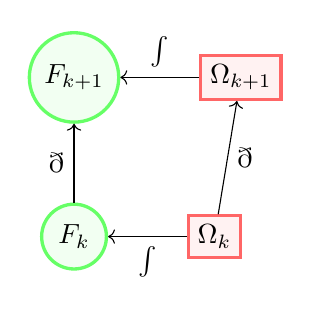
\begin{tikzpicture}
[roundnode/.style={circle, draw=green!60, fill=green!5, very thick, minimum size=7mm},
squarednode/.style={rectangle, draw=red!60, fill=red!5, very thick, minimum size=5mm},
]
\node[roundnode]	(f2) {$F_{k+1}$};
\node[roundnode]	(f1) [below=of f2]{$F_k$};
\node[squarednode]	(w2) [right=of f2] {$\Omega_{k+1}$};
\node[squarednode]	(w1) [right=of f1] {$\Omega_k$};

\draw[<-] (f2) -- (w2) node[midway, above] {$\int$};
\draw[<-] (f2) -- (f1) node[midway, left] {$\eth$};
\draw[<-] (f1) -- (w1) node[midway, below] {$\int$};
\draw[<-] (w2) -- (w1) node[midway, right] {$\eth$};
\end{tikzpicture}

- Remake this diagram using tikz (\textbf{Attempted, keeps being buggy. Deal with it later})



\begin{coro}
	\textbf{Stokes' Theorem}: For (k-1)-form $\omega$ and k-surface $\sigma$, $\int_{\partial \sigma}\omega = \int_{\sigma}\eth\omega$. 
\end{coro}

In many treatments of Electromagnetism (for example, "Classical Electromagnetic Radiation" by Heald and Marion), Stokes' Theorem is given in terms of the curl as \begin{gather}\int_S \nabla \times \vec{A} \cdot d\vec{S} = \oint_{\Gamma} \vec{A} \cdot d\vec{l}.\end{gather} This allows us to take a brief digression to see how the tools we have defined look in the more familiar 3D cases. 

We want to examine now how the exterior derivative explicity affects k-forms when written out in component form. In general, we have that for $\omega_k \in \Omega_k$, \begin{gather}\omega_k = \omega_{ab...c}e^a\wedge e^b \wedge ... \wedge e^c.\end{gather} It must be that an integral over the exterior derivative of a form results in one of the degrees of freedom being integrated away, putting the integral strictly on the boundary of the k-surface. [\textbf{Maybe show for 1D or 2D, since the general case is hard}]\begin{gather} \eth \omega_k = \partial_a\omega_{bc...d}e^a\wedge e^b\wedge e^c\wedge ... \wedge e^d.\end{gather} So, suppose we have $f \in \Omega_0$, $v \in \Omega_1$, and $B \in \Omega_2$, and we apply the exterior derivative to each of them. We have that \begin{gather}\eth f = \partial_a f e^a,\end{gather} \begin{gather}\eth v = \partial_a v_b e^a \wedge e^b,\end{gather} and \begin{gather}\eth B = \partial_a B_{bc} e^a\wedge e^b \wedge e^c.\end{gather} 

By looking closer at these expressions, we see familiar tools from vector calculus arise. $\partial_a f e^a$ is a 1-form consisting of the sum of derivatives in each of the basis directions. In the 3D case, we have that \begin{gather}\partial_a f e^a = \frac{\partial f}{\partial x^1} e^1 + \frac{\partial f}{\partial x^2} e^2 + \frac{\partial f}{\partial x^3} e^3.\end{gather} This is simply the gradient of a scalar functional. So, we have that in $\mathbb{R}^3$, \begin{gather}\partial_a f e^a = \nabla f.\end{gather} Similarly, we see that in 3D, $\eth v$ will give us a 2-form from a 1-form, composed of the sum of derivatives in the directions perpendicular to the original 1-form. That is, in $\mathbb{R}^3$, \textbf{[Explicitly show the algebra here]}\begin{gather}\eth v = (\frac{\partial v_2}{\partial x^3} - \frac{\partial v_3}{\partial x^2})e^2\wedge e^3 - (\frac{\partial v_1}{\partial x^3} - \frac{\partial v_3}{\partial x^1})e^1 \wedge e^3 + (\frac{\partial v_1}{\partial x^2} - \frac{\partial v_2}{\partial x^1})e^1 \wedge e^2.\end{gather} Finally, [\textbf{Don't need to show the algebra, just say "similarly we can find that..."}]\begin{gather} \eth B = (\frac{\partial B_1}{\partial x^1} + \frac{\partial B_2}{\partial x^2} + \frac{\partial B_3}{\partial x^3})e^1\wedge e^2 \wedge e^3.\end{gather} We see here that $\eth v$ doesn't \emph{quite} give us $\nabla \times v$, and $\eth B$ doesn't \emph{quite} give us $\nabla \cdot B$. This discrepancy demonstrates the difference between the wedge product and the cross product. Had we done $\nabla \times v$, the first term would have been $(\frac{\partial v_2}{\partial x^3} - \frac{\partial v_3}{\partial x^2})e^1$. That is, in the direction perpendicular to $e^2\wedge e^3$. This is similarly true for the components in $e^1\wedge e^3$ and $e^1 \wedge e^2$. Furthermore, $\nabla \cdot B$ returns a scalar\footnote{Note however that $\nabla \cdot B$ doesn't even return a true scalar. Rather, it returns a pseudoscalar: $\frac{\rho}{\epsilon_0}$. The difference here is similar to the difference between vector and pseudovector: if you flip one of the coordinates, you get an extra minus sign in a pseudoscalar, but a scalar is left invariant. Pseudovectors are associated with surfaces, and pseudoscalars are associated with volumes (hence, charge \textit{density} $\rho$.)} (i.e., no direction), while $\eth B$ returns a volume in the $e^1 \wedge e^2 \wedge e^3$ "direction." This discrepancy is resolved by the introduction of the Hodge Dual Operator $*$, such that $*\eth v = \nabla \times v$ and $*\eth B = \nabla \cdot B$, but this is beyond us at the moment. What does hold immediately true is a generalization of the expression \begin{gather} \nabla \times \nabla V = 0\end{gather} for any scalar function $V$. For any form $\omega_k \in \Omega_k$, we have that \begin{gather} \eth\eth\omega_k = 0.\end{gather}


You may be asking now, "But what about $\nabla \times \nabla \times B$ for $B \in \Omega_1$? This gives us $\nabla (\nabla \cdot B) - \nabla^2 B$, which certainly isn't zero in general. Didn't we show just that curl is really just the exterior derivative of a one-form?" The issue is, once again, that the exterior derivative of a one form isn't \emph{quite} the same thing as a curl of a vector field. This discrepancy arises because of the difference between the wedge product $\wedge$ and the cross product $\times$. For two vectors $a$ and $b$, $a \times b$ gives a vector perpendicular to the two of them, while the wedge product deals only with the two original tangent vectors. 
\textbf{We can sstart the discussion of potentials, closed, and exact here. Or move this to the next section}

With these new, more general geometric expressions for gradient, curl, and divergence, their physical interpretations become immediately clear, simply from the notation. If we extend the flux example, we see that the gradient of a 0-form is simply the lengthwise flow in each possible dimension (three, in 3D), the curl of a 1-form is the planewise flow in each plane (still 3, in 3D), and the divergence of a 2-form is the flow outwards from a point per unit volume. 



\section{Closed and Exact Forms, and Potentials}

\textbf{NOTE: Closed form relates to potentials with a point taken out, or a divergenceless field. So, the magnetic field. Motivate it based on that. If the boundary functional of some function is zero always, then we can say that it is a closed functional. Correspondantly, we can say that if we have a functional that is the boundary functional of some other functional, we can say that it is an exact functional. Generalization of potentials is basically saying that any functional that is closed is also exact. Potentials lie in the fact that if a form is exact, it is also closed. If the boundary functional is zero. This would probably be better to talk about in integral form. Intuitively, things make more sense in the integral, rather than in the infinitesimal. Actually, the real definition of closed functional is that the functional is closed if its zero for all closed surfaces. If the boundary function is closed, then it is the boundary functional of some potential.}

\textbf{Distinction between closed and exact disappears in integral (finite) form}

\textbf{We want to be able to build things from the finite concepts first. So in chapter 1, build as much as possible in the finite case. The infinitesimal forms are the limit cases. That makes the finite case geometrical. You don't have to imagine tangent spaces, etc. You are closed if you are closed on surfaces down to a point.}

In our discussions of Work functionals in Chapter 1, there naturally arose a relationship between functionals on boundaries and conservative/non-conservative forces. We can expand on this relationship now by making use of forms and the exterior derivative. 

Suppose we have a 1-functional $W$, a 1-form $f$, and a 0-form $v$, such that $f = \eth v$, and suppose we have some line $\lambda$, such that $W(\lambda) = \int_\lambda f(d\lambda)$. We have that \begin{gather}\int_\lambda f(d\lambda) = \int_\lambda \eth v(d\lambda),\end{gather} which, by Stokes' Theorem, equals \begin{gather} \int_{\partial\lambda} v(d\partial\lambda).\end{gather}

\textbf{Integrating on the closed loop is directly integrating over the exterior derivative of a thing. Imposing lambda being closed becomes unnecessary with the right application of $\eth$}

Suppose now that $\lambda$ is a closed loop; that is, its starting and ending points are the same. So, if we want to integrate our form over the entirety of $\lambda$, we have that \begin{gather} \int_{\partial\lambda} v(d\partial\lambda) = 0,\end{gather} so we have finally that \begin{gather} W(\lambda) = 0.\end{gather} Therefore, if we have the starting and ending points of $\lambda$ be the same, it doesn't matter what path we take otherwise, we will always get zero. If we let $W$ be a work functional, just as in Chapter 1, we see that we have just come across path-independent work and, more importantly, conservative forces. In this case, $f$ is a conservative force, related to a scalar potential $v$ by $f = \eth v$. Recalling that the exterior derivative of a 0-form is the same thing as a gradient of a scalar vector field, we see that saying that $f = \eth v$ is equivalent to saying that $F = -\nabla V$, for some conservative force $F$ and scalar potential $V$. The fact that $f = \eth v$ is the very thing that makes $f$ conservative.  

\textbf{This would make more sense in the finite form.}

Now say we have a 1-form $A$ such that $\eth A = 0.$ While it is true in general that $\eth\eth\omega = 0$ for all forms $\omega$, it doesn't necessarily have to be the case that $A = \eth v$ for some 0-form $v.$ Consider, for instance, the field $A = A_x e_x + A_y e_y = \frac{-y}{x^2 + y^2} e_x + \frac{x}{x^2 + y^2} e_y$. $\frac{\partial A_x}{\partial y} - \frac{\partial A_y}{\partial x} = 0$ (making the exterior derivative zero; see (2.41)), but it is not the exterior derivative of any other form. There is also a discontinuity at the point $(x,y) = (0,0)$. In the language of vector calculus, this is a divergenceless field (meaning that there is no "sink"), like the magnetic field, or the vector potential in the Coulomb gauge.  

\textbf{PUT A PICTURE OF THE CLOSED FIELD HERE}

These two examples introduce two important classes of differential forms and their physical implications. We are able to relate conservative forces to forms that are the exterior derivative of other forms, and divergenceless fields to forms with no exterior derivative. If a form is the exterior derivative of another form, it is \textbf{exact}, and if a form has no exterior derivative, it is \textbf{closed}.
 
\begin{defn} 
	A k-form \textbf{$\omega$} is \textbf{closed} if $\eth\omega = 0$. 
\end{defn}

\begin{defn} 
	A k-form \textbf{$\omega$} is \textbf{exact} if there exists a (k-1)-form $\alpha$ such that $\omega = \eth\alpha$.
\end{defn}



It follows from this that all exact forms are closed (since $\eth\eth\omega = 0$ for all forms). But once again, not all closed forms are exact, such as in the case of the $A$ field above. However, a region may be constructed such that the closed form is \emph{locally} exact. The only requirement to this region is that it does not include the discontinuity, the origin. Therefore, a potential exists in that local region. Thus, a field may be locally conservative, even if it is not globally conservative. 




\textbf{NOTE: In fluid dynamics for divergenceless fluid, there's something called stream functions}

\textbf{Bohm: If the form is closed, then the exterior derivative is always zero, thus all the integrals on closed surface that can be shrunk to a point will be zero. So, taking a convex region, we can create a potential there. z.B. assume we have a line}

\textbf{If it happens that the number for all closed surfaces (small enough up to a certain point) are always zero, then the form/functional is cosed. If it's zero on all the closed k-surfaces we give it, then its exact. The difference is that both admit potentials, but the closed form is only going to admit a potential in a convex region small enough where al the closed surfaces are zero. The exact will admit a potential globally (an n-1 form/functional that if given the exterior derivative gives the original thing)}

\textbf{Closed if for some set, all closed surfaces give zero for the functional. Exact if that open region corresponds to the whole space. Closed implies exact, but not the other way around}
















\end{document}